\documentclass[12pt, openany]{report}

\usepackage[utf8]{inputenc}
\usepackage[T1]{fontenc}
\usepackage[a4paper,left=2cm,right=2cm,top=2cm,bottom=2cm,headheight = 15pt]{geometry}
\usepackage{libertine}
\usepackage[pdftex]{graphicx}
\usepackage{totpages}
\usepackage[hidelinks]{hyperref}

\usepackage{helvet}
\renewcommand{\familydefault}{\sfdefault}
\usepackage[english, french]{babel}
\usepackage{subcaption}

\usepackage{setspace}
\onehalfspacing

% Change l'espacement entre deux paragraphes
\setlength{\parskip}{18pt}

% Liste à puces
\frenchbsetup{StandardLists=true}

% Édite style sous-titre figure et tableau
\usepackage[font=it]{caption}

% Change l'en-tête et le pied de page pour tout le document
\usepackage{fancyhdr}
\pagestyle{fancy}

\renewcommand{\chaptermark}[1]{\markboth{\thechapter.\ #1}{}}
\renewcommand{\sectionmark}[1]{\markright{\thesection.\ #1}}

\renewcommand{\headrulewidth}{0.5pt} 
\fancyhead[L]{\bfseries\leftmark}
\fancyhead[C]{}
\fancyhead[R]{\rightmark}

\renewcommand{\footrulewidth}{0.5pt}
\fancyfoot[L]{\textbf{Tugdual Le Pen}}
\fancyfoot[C]{}
\fancyfoot[R]{\thepage\ / \ref{TotPages}}

\fancypagestyle{plain}{ %
    \fancyhf{} % remove everything

    \renewcommand{\headrulewidth}{0pt} 
    \renewcommand{\footrulewidth}{0.5pt}
    \fancyfoot[L]{\textbf{Tugdual Le Pen}}
    \fancyfoot[C]{}
    \fancyfoot[R]{\thepage\ / \ref{TotPages}}
}

% Change le style des parties et sous partiess
\usepackage[explicit]{titlesec}
% change l'espacement au niveau du titre des chapitres
\titlespacing*{\chapter}
  {0pt}%  indent
  {0pt}% space before
  {12pt}% space after

\titlespacing*{\section}
  {0.6cm}%  indent
  {0pt}% space before
  {0pt}% space after

% Définie les couleurs utilisées dans le rapport
\usepackage{color}

\definecolor{darkblue}{rgb}{0.11, 0.30, 0.66}
\definecolor{lightblue}{rgb}{0.18, 0.42, 0.86}
\definecolor{gray}{rgb}{0.4,0.4,0.4}
\definecolor{black}{rgb}{0.0,0.0,0.0}
\definecolor{green}{rgb}{0.4, 0.8, 0.2}

%% Style Chapitre
% -------------------------------------------------------
% Avec numéro
\titleformat{\chapter}[hang] 
    {\fontsize{24pt}{0pt}\selectfont \bfseries}
    {\textcolor{darkblue} 
    {\thechapter. #1}}
    {0pt}
    {\huge}

% Sans numéro
\titleformat{name=\chapter,numberless}[hang] 
    {\fontsize{24pt}{0pt}\selectfont \bfseries}
    {\textcolor{darkblue} 
    {#1}}
    {0pt}
    {\huge}
% -------------------------------------------------------

%% Style Section
% -------------------------------------------------------
% Avec numéroté
\titleformat{\section}[hang]
    {\fontsize{16pt}{0pt}\selectfont \bfseries}
    {\textcolor{lightblue} 
    {\thesection.\ #1}}
    {10pt}
    {\Large}

% Sans numéro
\titleformat{name=\section,numberless}[display] 
    {\fontsize{16pt}{0pt}\selectfont \bfseries}
    {\textcolor{lightblue} 
    {\thechapter.\thesection #1}}
    {10pt}
    {\Large}
% -------------------------------------------------------

% Numérotation des chapitre en chiffre Romain
\renewcommand{\thechapter}{\Roman{chapter}}

% Créer commande pour lien url
\newcommand{\link}[1]{{\color{lightblue}\href{#1}{#1}}}

% Éviter les orphelin en début ou fin de page
\widowpenalty=10000 
\clubpenalty=10000 
\raggedbottom

% Nouvelle commande pour ajouter des commentaire sur le rapport
\newcommand{\comment}[1]{\emph{\color{green} \% #1}}



\begin{document}
\selectlanguage{french}
% Édite style sous-titre image et tableau
\makeatletter
\newcommand{\figcapfont}{\itshape} 
\newcommand{\tabcapfont}{\itshape}
\renewcommand{\fnum@figure}{\figcapfont Image \thefigure}
\renewcommand{\fnum@table}{\tabcapfont Tableau \thetable}
\makeatother

\begin{titlepage}
  \begin{center}

    % Logo Esir and Irisa
    % Author and supervisor
    \begin{minipage}{0.45\textwidth}
      \begin{flushleft} \large
        
\includegraphics[width=0.9\columnwidth]{datas/logo_esir.jpg}~\\
        \emph{Élève-ingénieur :}\\
        Tugdual Le Pen\\
        Imagerie Numérique\\
        2\up{ème} année du cursus ingénieur\\
        ~\\
        \emph{Tuteur universitaire :}\\
        Pierre Maurel\\
        Enseignant chercheur
      \end{flushleft}
    \end{minipage}
    \begin{minipage}{0.45\textwidth}
      \begin{flushright} \large
        \vspace{19pt}
        
\includegraphics[width=0.9\columnwidth]{datas/logo_irisa.jpg}~\\~\\
        IRISA\\
        263 Avenue du Général Leclerc\\
        35000 RENNES - France\\
        contact@irisa.fr\\
        ~\\        
        \emph{Tuteur organisation :}\\
        Olivier Le Meur\\
        Enseignant chercheur\\
      \end{flushright}
    \end{minipage}

    \vspace{4cm}

    \textsc{\Huge \textbf{Titre du rapport de stage}}\\[28pt]    

    \vfill

    % Bottom of the page
    \begin{minipage}{0.45\textwidth}
      \begin{flushleft}
        \vspace{0.5cm}
        {\large Année universitaire 2019 - 2020}
      \end{flushleft}
    \end{minipage}
    \begin{minipage}{0.45\textwidth}
      \begin{flushright}
        
\includegraphics[width=0.9\columnwidth]{datas/logo_univ.png}~\\
      \end{flushright}
    \end{minipage}

  \end{center}
\end{titlepage}

% Actualise le compteur de page
\clearpage
\setcounter{page}{2}

\chapter{Remerciements}
\par
    Je tiens dans un premier temps à exprimer ma gratitude à l'IRISA et plus particulièrement à l'équipe Percept pour m'avoir accueilli et considéré en tant que collaborateur durant ces six mois de stage.
\vspace{24pt}
\par
    Je remercie mon tuteur Olivier Le Meur pour sa pédagogie, sa confiance et son savoir-faire qui m'ont permis d'avancé sur mon projet serainement et efficacement.
\vspace{24pt}
\par
    Merci également aux doctorants et ingénieurs de l'équipe Percept avec qui j'ai pu échanger des bons moments et des conseils précieux pour le développement de mon projet.
\vspace{24pt}
\par
    Je désire aussi aussi remercier les professeurs de l‘Ecole Supérieure d'ingénieurs de Rennes, qui m’ont fourni les outils nécessaires au bon déroulement de mon stage. Je tiens à remercier spécialement Pierre Maurel mon professeur référent universitaire.

\vspace{24pt}
\par
    Enfin, pour conclure, je souhaiterais remercier toutes les personnes qui ont participé de différentes façons à la réussite de mon stage.

\addcontentsline{toc}{chapter}{Résumé}
\chapter*{Résumé}
\par
    Pour valider ma 4\up{ème} année de mon cycle ingénieur en Technologie de 
    l'Information avec spécialité Imagerie Numérique, j'ai effectué un stage 
    d'une durée de six mois dans l'Institut de Recherche en Informatique et 
    Systèmes Aléatoires (IRISA). C'est un laboratoire de recherche impliqué dans 
    le domaine de l'informatique et des technologies de l'information. Il couvre 
    l'ensemble des thématiques de ces domaines, de l’architecture des 
    ordinateurs et des réseaux à l’intelligence artificielle en passant par le 
    génie logiciel, les systèmes distribués et la réalité virtuelle.

\par
    J'ai rejoint plus précisément l'équipe Percept (2018) qui est spécialisée 
    dans le comportement visuel de différentes populations. L'un des projets de 
    cette équipe est d'étudier la saillance dans les peintures. Notamment la capacité 
    de déterminer cette saillance automatiquement au moyen de machine learning.

\par
    Mon objectif est de participer à ce projet et mettre en place des 
    applications qui permettraient de montrer les possibiltés d'utilisations de 
    ce genre de programme.

\vspace{40pt}

\selectlanguage{english}
\color{gray}
\par
    To validate my 4\up{th} year of my engineer cycle specializing in Digital 
    Imaging, I did a six-month internship in the Research Institute in Computer 
    Science and Random Systems (IRISA). It is a research laboratory involved in 
    the field of computer science and information technology. It covers all the 
    themes of these fields, from the architecture of computers and networks to 
    artificial intelligence, including software engineering, distributed systems 
    and virtual reality. 

\par
    I joined the team Percept (2018) which specializes in the visual behavior of 
    different populations. One of the projects of this team is to study the 
    saliency in paintings. In particular the ability to determine this salience 
    automatically by means of machine learning. 

\par
    My objective is to participate in this project and set up applications which 
    allow us to show the possibilities of uses of this kind of program.

\selectlanguage{french}
\color{black}

% Renomme "Tables des matières" en "Sommaire"
\renewcommand{\contentsname}{Sommaire}
{\setlength{\parskip}{6pt}
\tableofcontents
}

\chapter{Introduction}

% rapide résumé contexte, explication du sujet et pk avoir choisi le stage

%Intro contexte
\par
La peinture et le mouvement du regard de l'Homme ont toujours eu un lien étroit. En effet chaque spectateur regardera un tableau d'une manière différente de son voisin parce que chaque individu a sa propre culture, son propre point de vue... Pourtant la structure d'une peinture amènera le spectateur à suivre un sens de lecture. Celui-ci sera généralement commun à tous les spectateurs. Par exemple un individu qui découvre le tableau de La Joconde pour la première fois regardera presque systématiquement en premier lieu le visage de Mona Lisa et particulièrement ces yeux qui ont un effet particulier. Rare sont les personnes qui commenceront par identifier les éléments du décor en arrière-plan de la peinture.

\begin{figure}[h]
    \centering
    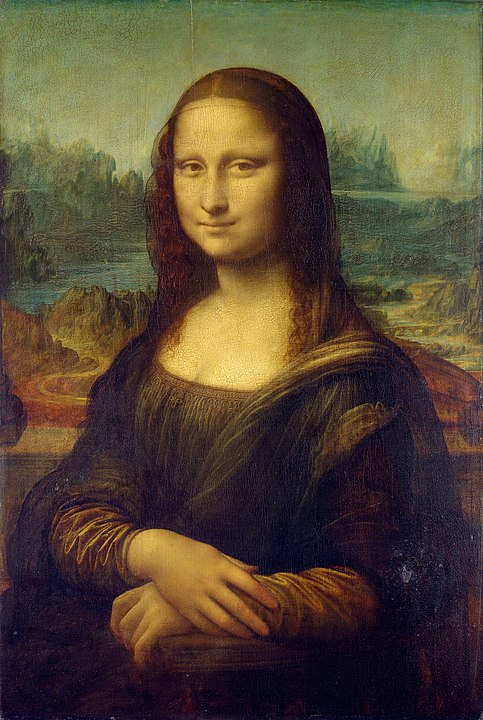
\includegraphics[width=0.3\textwidth]
                    {datas/Mona_Lisa_by_Leonardo_da_Vinci.jpg}
    \caption{La Joconde de Leonard de Vinci}
\end{figure}

%Intro saillance, Irisa et percept
\par
Ce sont l'ensemble de ces éléments qui attirent l'\oe{}il humain qui constituent la saillance. C'est un élément important pour de nombreux domaines. On pense notamment au domaine du marketing et de la publicité qui doivent créer des affiches ou des spots publicitaires avec pour objectif d'attirer le plus possible le regard des consommateurs.

%Intro 
\par
La saillance dans la peinture permet d'analyser et de comprendre le regard humain ainsi que toutes les particularités qui en découlent. L'équipe Percept, équipe de recherche du laboratoire de l'IRISA, se penche sur le sujet et notamment à l'automatisation pour déterminer la saillance dans les peintures à l'aide de modèles de réseaux de neurones basés sur le machine learning.

%Explication du sujet de stage
\par
C'est là que le sujet de mon stage intervient. Cela consiste dans un premier temps à faire l'état de l'art des différents modèles de saillance qui existent sur des images naturelles. Dans un second temps le but est d'adapter le meilleur modèle pour qu'il s'adapte à des peintures. Et enfin à partir des résultats de ce modèle trouver des applications visuelles et ludiques pour montrer l'intérêt d'un tel modèle.

%Explication comment j'ai trouvé le stage et quelles étaient mes motivations
\par 
Ce stage qui m'as été proposé par Olivier Le Meur correspondait à ce que je recherchais. C'est-à-dire un stage basé sur le machine learning, qui fait suite à mon projet industriel à l'ESIR qui consistait à générer des visages au moyen de réseau de neurones antagoniste génératif (GAN). Mais aussi un stage varié qui puisse me permettre de me former sur plusieurs compétences différentes.
% en conclusion : J'ai aimé la liberté et l'autonomie du stage, notamment les discussions qu'on a pu avoir avec Olivier pour déterminer quelles seraient les futur étapes du projet.

\chapter{IRISA}

\par
L'IRISA - Institut de Recherche en Informatique et Systèmes Aléatoires - est
aujourd'hui le plus grand laboratoire de recherche français (+ de 850 personnes)
dans le domaine de l'informatique et des technologies de l'information. Il
couvre l'ensemble des thématiques de ces domaines, de l'architecture des
ordinateurs et des réseaux à l'intelligence artificielle en passant par le génie
logiciel, les systèmes distribués et la réalité virtuelle.

\par
L'IRISA est issu d'une volonté de collaboration entre huit établissements tutelles pluridisciplinaires : CentraleSupélec, CNRS, ENS Rennes, IMT Atlantique, Inria, INSA Rennes, Université Bretagne Sud, Université de Rennes 1.

\begin{figure}[h]
    \centering
    
\includegraphics[width = 0.7\textwidth]{datas/logo_irisa.jpg}
    \caption{Logo de l'IRISA}
\end{figure}

\par
l'IRISA est présent sur 3 sites géographiques au sein du territoire breton (Rennes, Lannion, Vannes). Mon stage s'est déroulé dans les locaux de Rennes.
Le laboratoire est structuré en sept départements scientifiques :
\begin{itemize}
    \item D1 - Systèmes Large Échelle
    \item D2 - Réseaux, Télécommunication et Services
    \item D3 - Architecture
    \item D4 - Langage et génie logiciel
    \item D5 - Signaux et Images numériques, Robotique
    \item D6 - Média et interactions
    \item D7 - Gestion des données et dela connaissance
\end{itemize}


\par
L'équipe PERCEPT du département Média et intéractions est spécialisé dans le comportement visuel de différentes populations.

\bibliographystyle{plain}
\addcontentsline{toc}{chapter}{Bibliographie}
\begin{thebibliography}{99}

	\bibitem{irisa}
	  Site de l'IRISA - Présentation du laboratoire\\
      \link{https://www.irisa.fr/fr/page/recherche-innovation-sciences-technologies-du-numerique}
      
      \bibitem{percept}
	  Site de l'IRISA - Présentation de l'équipe PERCEPT\\
      \link{https://www.irisa.fr/fr/equipes/percept}

      \bibitem{gaze}
      \emph{Art, Aesthetics, and the brain}, 2015\\
      par J.P. Huston, M. Nadal, F. Mora, L.F. Agnati et C.J. Cela-Conde

      \bibitem{benchmark_MIT}
      \emph{Mit saliency benchmark}, 2015\\
      par Bylinskii Z, Judd T, Borji A, Itti L, Durand F, Oliva A, et al.

\end{thebibliography}


\appendix
\addcontentsline{toc}{chapter}{Annexes}
\chapter*{Annexes}


\end{document}

% Plan :
% Page de garde -- Done
% Remerciements -- Done
% Résumé (anglais français) -- Done
% Sommaire -- Done
% Introduction
%%% rapide résumé contexte, entreprise, explication du sujet et pk avoir choisi le stage
% Présentaion Irisa et mission de stage
% Analyse du problème et de son contexte / étude de l'existant / méthode et plan de travail
%%% Introduction à la saillance et au machine learning
% Solution proposée / Travail réalisé / Résultats développés
%%% prise en main de python et de la saillance : video fondu et scanpath
%%% diapo pour journée du patrimoine irisa
%%% puis benchmark des differents algo
%%% puis finetuning de SAM-RESNET (the best)
%%% appli : ken burns video + ...
% évaluation / Interprétation des résultats / Retour d'expérience / Bilan
%%% finetuning a permis de faire un papier (accepter par plosone ?)
% Conclusion
% Biblio
% Annexes


